\chapter{From Initial Data to Least Action}

These notes follow Leonard Susskind's second lecture on classical mechanics, as preserved in the course recording curated by LazyingArt LLC and Video2Book. The lecture begins as review, but the review is tactical: a deliberately false law is used to expose what the order of a differential equation really means, then Newtonian mechanics is recovered, and only after that do energy, momentum, and finally the principle of least action come into view. The movement is from local data to global trajectories, and it is worth preserving that progression carefully.

\section{First-Order Versus Second-Order Dynamics}

We begin with the initial-data problem in the simplest setting: one-dimensional motion. The point is not history, but the structure of the equations. Susskind introduces a false law, ``Aristotle's law,''
\begin{equation}
F=m\dot x,
\end{equation}
and, with the additional assumption that the force is a known function of position,
\begin{equation}
F(x)=m\dot x.
\end{equation}
This law is physically wrong, but mathematically it is perfectly consistent. That is precisely why it is useful here.

If we know the position \(x\) at one instant, then the force \(F(x)\) is immediately known. But then the equation itself tells us \(\dot x\). In other words, for a first-order law of this kind, position already determines velocity. We can push this further. Differentiate with respect to time:
\begin{align}
m\ddot x &= \frac{dF}{dt}
= \frac{dF}{dx}\,\dot x.
\end{align}
So if \(x\) is known, then \(F(x)\) is known, hence \(\dot x\) is known, and therefore \(\ddot x\) is known as well. Differentiate once more:
\begin{align}
m\dddot x
&= \frac{d}{dt}\!\left(\frac{dF}{dx}\,\dot x\right)
= \frac{d^2F}{dx^2}\,\dot x^{\,2} + \frac{dF}{dx}\,\ddot x.
\end{align}
Now the jerk \(\dddot x\) is also determined by the position. The pattern is clear: each further derivative is obtained from the preceding ones and from derivatives of the force law. A first-order equation closes immediately. If the initial position is given, the whole motion is, in principle, already fixed.

Newton's law behaves differently:
\begin{equation}
F(x)=m\ddot x.
\end{equation}
If we know the position at \(t=0\), then we know the force, and therefore the acceleration. But the equation does not tell us the velocity. The missing datum is real. A second-order law needs both \(x\) and \(\dot x\) at the starting time. Once those are supplied, the force law determines \(\ddot x\), and from there one can continue to higher derivatives exactly as before.

That is the first real conclusion of the lecture: Newtonian mechanics is second order in time, and therefore its initial conditions consist of positions and velocities, not positions alone.

\subsection{Question \& Answer}

\paragraph{Question.} Why does Newton need both position and velocity while Aristotle's law did not?

\paragraph{Answer.} Because the difference is not a detail of the force law; it is the order of the differential equation. In a first-order law such as \(F(x)=m\dot x\), the position determines the first derivative directly. In Newton's law \(F(x)=m\ddot x\), the position determines only the second derivative. Velocity is therefore an independent piece of initial data. The physics is different because the mathematical order is different.

\section{Conservative Forces and Energy Conservation}

From the initial-data problem the lecture turns to conservation of energy. Here Susskind is careful to lower our expectations and raise them at the same time. The proof he is about to give is elementary, but the principle itself is deeper than the proof. Energy conservation survives in electromagnetism, relativity, and quantum mechanics; Newton's equations are only the temporary stage on which the result is being reviewed.

He first reminds us that not every force law conserves the naive sum of kinetic and potential energy. Friction, if treated only macroscopically, seems to destroy mechanical energy. A force that keeps pushing a particle around a circle in the same direction would increase its speed on each circuit without changing its position, so no ordinary potential energy could compensate for the gain in kinetic energy. The forces that do lead to the usual conservation law are conservative forces.

For a single particle, possibly in several spatial dimensions, the conservative-force law is
\begin{equation}
F_i=-\frac{\partial U}{\partial x_i},
\qquad
\mathbf F=-\nabla U.
\end{equation}
The minus sign matters: force points toward decreasing potential energy.

\begin{figure}[h]
\centering

\includegraphics[width=0.52\textwidth]{lecture_02_figure_02.png}
\caption{Energy definition and separate time-derivative terms. The top handwritten symbol is best read as \(T\), in agreement with the transcript and the logic of the derivation.}
\end{figure}

We then define the kinetic and total energies by
\begin{equation}
T=\frac12 mv^2=\frac12 m\sum_i v_i^2,
\qquad
E=T+U.
\end{equation}
The board in the lecture sets these ingredients up one by one before allowing them to combine.

\begin{figure}[h]
\centering

\includegraphics[width=0.78\textwidth]{lecture_02_figure_03.png}
\caption{Combined time derivative of the total energy and the force-minus-force cancellation.}
\end{figure}

Now for the derivation. Since \(m\) is constant,
\begin{align}
\frac{dT}{dt}
&= \frac{d}{dt}\left(\frac12 m\sum_i v_i^2\right)
= \sum_i m v_i \frac{dv_i}{dt}
= \sum_i m v_i a_i.
\end{align}
For the potential energy, which is a function of the coordinates,
\begin{align}
\frac{dU}{dt}
&= \sum_i \frac{\partial U}{\partial x_i}\frac{dx_i}{dt}
= \sum_i \frac{\partial U}{\partial x_i}v_i.
\end{align}
Add them:
\begin{align}
\frac{dE}{dt}
&= \frac{dT}{dt}+\frac{dU}{dt} \\
&= \sum_i \left(m a_i+\frac{\partial U}{\partial x_i}\right)v_i.
\end{align}
Now use Newton's law \(m a_i=F_i\) and the conservative-force form \(\partial U/\partial x_i=-F_i\). Then
\begin{align}
\frac{dE}{dt}
&= \sum_i (F_i-F_i)v_i
=0.
\end{align}
So the total energy is conserved.

The important point in the lecture is not merely the algebra, but the order of the algebra. First the pieces are written down, then differentiated separately, then grouped into a single expression, and only then does the cancellation appear. The proof is review, but the conservation law already hints that there is a more general structure waiting behind Newton's equations.

\section{Momentum and Closed Systems}

The lecture now changes emphasis rather than subject. Newton's law is rewritten, not replaced:
\begin{equation}
F_i = m\frac{dv_i}{dt}.
\end{equation}
Because the mass is constant, we can pull it into the derivative,
\begin{equation}
F=\frac{d}{dt}(mv),
\end{equation}
and if we name the quantity \(mv\) by
\begin{equation}
\vec P = m\vec v,
\end{equation}
then Newton's law becomes
\begin{equation}
\vec F=\frac{d\vec P}{dt}.
\end{equation}

\begin{figure}[h]
\centering

\includegraphics[width=0.52\textwidth]{lecture_02_figure_04.png}
\caption{Newton's law being rewritten in momentum form. This is a transition frame rather than a final formula plate, but it preserves the live movement of the board.}
\end{figure}

\begin{figure}[h]
\centering

\includegraphics[width=0.52\textwidth]{lecture_02_figure_05.png}
\caption{Component and vector forms of force and momentum.}
\end{figure}

The lecture pauses here for a worthwhile question: what assumptions about time are already built into this Newtonian picture? The answer is explicit. We are assuming a universal synchronized time, common to all points in space, and we are also assuming, for the moment, that the force law has no explicit time dependence. This is the naive Newtonian framework, and Susskind wants it named before momentum conservation is derived inside it.

For a closed many-particle system, the force on each particle is the sum of the forces due to the others. With three particles,
\begin{align}
\vec F_1 &= \vec F_{12}+\vec F_{13}, \\
\vec F_2 &= \vec F_{21}+\vec F_{23}, \\
\vec F_3 &= \vec F_{31}+\vec F_{32}.
\end{align}
Here the notation is important: \(\vec F_{12}\) means the force on particle \(1\) due to particle \(2\). Newton's third law gives the equal-and-opposite relations
\begin{equation}
\vec F_{12}=-\vec F_{21},
\qquad
\vec F_{13}=-\vec F_{31},
\qquad
\vec F_{32}=-\vec F_{23}.
\end{equation}
Since \(\dot{\vec P}_i=\vec F_i\), we have
\begin{align}
\frac{d\vec P_1}{dt} &= \vec F_{12}+\vec F_{13}, \\
\frac{d\vec P_2}{dt} &= \vec F_{21}+\vec F_{23}, \\
\frac{d\vec P_3}{dt} &= \vec F_{31}+\vec F_{32}.
\end{align}
Adding,
\begin{align}
\frac{d}{dt}\bigl(\vec P_1+\vec P_2+\vec P_3\bigr)
&= \vec F_{12}+\vec F_{13}+\vec F_{21}+\vec F_{23}+\vec F_{31}+\vec F_{32} \\
&= 0.
\end{align}
Therefore
\begin{equation}
\frac{d\vec P_{\text{tot}}}{dt}=0.
\end{equation}
That is momentum conservation for a closed system.

\begin{figure}[h]
\centering

\includegraphics[width=0.78\textwidth]{lecture_02_figure_06.png}
\caption{Pairwise force sketch for momentum conservation. The board drawing is qualitative; the transcript controls the exact force labels.}
\end{figure}

\begin{figure}[h]
\centering
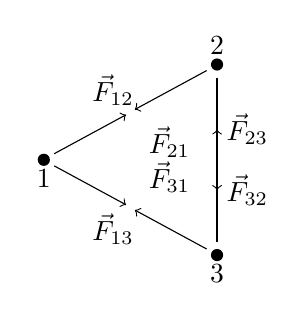
\begin{tikzpicture}[scale=1.1]
\fill (0,0) circle (2pt) node[below] {$1$};
\fill (2,1.1) circle (2pt) node[above] {$2$};
\fill (2,-1.1) circle (2pt) node[below] {$3$};

\draw[->] (0.12,0.07) -- (0.95,0.52);
\draw[->] (1.88,1.03) -- (1.05,0.58);
\node at (0.8,0.8) {$\vec F_{12}$};
\node at (1.45,0.2) {$\vec F_{21}$};

\draw[->] (0.12,-0.07) -- (0.95,-0.52);
\draw[->] (1.88,-1.03) -- (1.05,-0.58);
\node at (0.8,-0.8) {$\vec F_{13}$};
\node at (1.45,-0.2) {$\vec F_{31}$};

\draw[->] (2,0.95) -- (2,-0.35);
\draw[->] (2,-0.95) -- (2,0.35);
\node at (2.35,0.35) {$\vec F_{23}$};
\node at (2.35,-0.35) {$\vec F_{32}$};
\end{tikzpicture}
\caption{A cleaned pairwise-force diagram clarifying the cancellation of internal forces.}
\end{figure}

\subsection{Question \& Answer}

\paragraph{Question.} Are action and reaction instantaneous, and which part of the argument is specifically Newtonian?

\paragraph{Answer.} In Newtonian mechanics, yes: action and reaction are taken to be instantaneous because time is assumed universal and signal propagation effectively infinite. That assumption is specifically Newtonian. But the lecture is careful about the deeper lesson. Special relativity removes instantaneous force propagation, yet momentum conservation survives. So the toy derivation above is Newtonian; the conservation law itself is more general.

\section{From Local Laws to Whole Trajectories}

At this point the lecture makes its major turn. Newton's equations are local equations along a trajectory. If we know where the system is and how it is moving at one time, then the force law tells us the acceleration, and therefore tells us how to move one step further. The whole trajectory is built point by point.

To describe a general mechanical system, we introduce generalized coordinates,
\begin{equation}
q_1,\ q_2,\ \dots,\ q_n,
\end{equation}
which may be Cartesian coordinates, angles, orientations, or any other variables that specify the configuration. The motion is then described by the whole collection of functions
\begin{equation}
q_1(t),\ q_2(t),\ \dots,\ q_n(t).
\end{equation}
That collection is the generalized trajectory of the system.

In the Newtonian formulation, the initial-data problem asks for the trajectory given the coordinates and velocities at one time:
\begin{equation}
q_i(t_0),\qquad \dot q_i(t_0).
\end{equation}
For a second-order theory, that is the right amount of information. But there is another way to pose the same problem. Instead of giving position and velocity at one time, we may give the positions at two distinct times, say at \(t_0\) and \(t_1\). Then we ask for the trajectory connecting those endpoints.

This is the hinge of the lecture. The local Newtonian picture propagates the motion from instant to instant. The least-action picture will instead assign a number to the entire path and select the physically realized path globally. The physics is the same; the formulation is not.

\section{Stationary Points and Ordinary Functions}

Before dealing with trajectories, the lecture pauses for a mathematical warm-up. If \(f(y)\) is an ordinary function of one variable, then a local minimum, maximum, or inflection point all share the same first condition:
\begin{equation}
\frac{df}{dy}=0.
\end{equation}
That condition is not enough to distinguish minima from maxima, but it is enough to locate the points where the function is stationary.

This distinction matters because the principle of least action is, more precisely, a principle of stationary action. Susskind says quite openly that he will usually keep the simpler phrase ``least action,'' but he wants us to know what has been given up in the simplification.

For several variables the condition generalizes in the obvious way. If
\begin{equation}
f=f(x_1,\dots,x_n),
\end{equation}
then a stationary point must satisfy
\begin{equation}
\frac{\partial f}{\partial x_i}=0
\qquad \text{for every } i.
\end{equation}

The lecture works through a two-variable example:
\begin{equation}
f(x,y)=x^2+y^2+3x+2y+xy+7.
\end{equation}
The stationary-point equations are
\begin{align}
\frac{\partial f}{\partial x} &= 2x+y+3=0, \\
\frac{\partial f}{\partial y} &= x+2y+2=0.
\end{align}
The structural point is the important one: the constant \(7\) drops out, and a function of two variables gives two equations for two unknowns. If one solves these equations carefully, one finds
\begin{equation}
x=-\frac43,\qquad y=-\frac13,
\end{equation}
although in the lecture itself the arithmetic is treated as secondary to the method.

\subsection{Question \& Answer}

\paragraph{Question.} Is the principle really least action, or stationary action?

\paragraph{Answer.} Strictly speaking it is stationary action. The first-order variation must vanish, and that condition includes minima, maxima, and certain inflection-type cases. In ordinary mechanical problems one often does encounter a true minimum, and the lecture is content to speak that way, but the mathematically correct phrase is ``stationary action.''

\section{Functionals: Least Distance and Least Time}

We are now ready to minimize not a function of finitely many variables, but a quantity that depends on an entire curve. This is the transition to the calculus of variations.

Take a curve \(y(x)\) connecting two fixed endpoints. For a small segment of the curve,
\begin{equation}
ds^2 = dx^2+dy^2,
\end{equation}
so
\begin{equation}
ds=dx\sqrt{1+\left(\frac{dy}{dx}\right)^2}.
\end{equation}
Integrating from \(x_1\) to \(x_2\), we obtain the total arc length
\begin{equation}
s_{12}[y]
=
\int_{x_1}^{x_2}
\sqrt{1+\left(\frac{dy}{dx}\right)^2}\,dx.
\end{equation}
This is not a function of a few numbers. It is a rule that takes a whole function \(y(x)\) as input and returns a number. That is a functional.

There are two viewpoints here, and the lecture insists on both. Globally, we minimize the total length of the entire curve. Locally, if we zoom into a tiny segment, the condition for minimal distance is simply: go straight ahead. The local and global viewpoints are different formulations of the same geometric truth.

The optical example is the principle of least time. Suppose the speed of light depends on height, \(c=c(y)\). Then
\begin{equation}
c(y)=\frac{ds}{dt},
\qquad
dt=\frac{ds}{c(y)}.
\end{equation}
Substituting the expression for \(ds\),
\begin{equation}
dt
=
\frac{\sqrt{1+\left(\frac{dy}{dx}\right)^2}}{c(y)}\,dx.
\end{equation}
Therefore the total travel time is the functional
\begin{equation}
t_{12}[y]
=
\int_{x_1}^{x_2}
\frac{\sqrt{1+\left(\frac{dy}{dx}\right)^2}}{c(y)}\,dx.
\end{equation}
Now the path is no longer generally a straight line. If light moves faster in higher layers of the medium, the minimizing path may bend upward to spend more of its travel in the faster region. The lecture's point is not to solve that problem here, but to establish the form of the problem: fixed endpoints, a whole curve, and a functional whose stationary value selects the physical path.

\section{Generalized Coordinates and the Action}

With the variational language in place, the lecture returns to mechanics. The endpoint formulation now takes center stage: instead of initial position and velocity, we specify the configuration at the beginning and at the end of the time interval, and we ask for the trajectory that connects them.

For one particle in one dimension, the unknown trajectory is \(x(t)\). Since the lecture has just trained us to expect a functional of a whole path, it is natural to ask what quantity is to be minimized. A naive guess would be the time integral of the total energy,
\begin{equation}
\int_{t_0}^{t_1} (T+U)\,dt.
\end{equation}
Susskind pauses here precisely to let that guess form, because the correction is the surprise: the right combination is not \(T+U\), but \(T-U\).

So the action is
\begin{equation}
A[x]
=
\int_{t_0}^{t_1}
\left(
\frac12 m\dot x^{\,2}-U(x)
\right)\,dt.
\end{equation}
The integrand is called the Lagrangian,
\begin{equation}
L = T-U.
\end{equation}
For a general Newtonian mechanical system this becomes
\begin{equation}
L(q,\dot q)=T-U,
\qquad
A[q]=\int_{t_0}^{t_1}L(q,\dot q)\,dt.
\end{equation}
The lecture also emphasizes the dependence structure: just as the optical time functional depends on both \(y(x)\) and \(dy/dx\), the action depends on the coordinates \(q_i(t)\) and on their time derivatives \(\dot q_i(t)\).

Susskind also remarks on notation. Since \(s\) has already been used for path length, it is better not to use \(s\) for the action here. The real content, however, is not the letter. It is the claim that every mechanical system admits a Lagrangian, and that the realized trajectory is the one that makes the action stationary.

\subsection{Question \& Answer}

\paragraph{Question.} Why is the action built from kinetic minus potential energy rather than the total energy?

\paragraph{Answer.} At the level of this lecture, the honest answer is: because that is the combination that reproduces Newton's equations when the variational principle is worked out. The lecture does not try to motivate the minus sign from first principles before the calculation; it postpones that deeper explanation. But once the potential is defined by \(F=-dU/dx\), the sign is no longer cosmetic. The variational principle built from \(T-U\) yields the Newtonian force law with the correct sign, whereas the naive \(T+U\) does not.

There is also a broader remark. In Newtonian particle mechanics the Lagrangian is \(T-U\), but the lecture already signals that in more general systems the Lagrangian may be a different function of \(q\) and \(\dot q\). The deeper principle is not the special formula \(T-U\) by itself, but the existence of a stationary action.

The lecture ends deliberately at this threshold. We are told what the action is, but not yet how to vary it. The next step will be to derive the equations of motion from the action and show that, in the Newtonian cases under discussion, they are equivalent to Newton's equations.

\section{Summary}

The lecture begins with initial data and ends with the action, but the path between them is carefully staged. A false first-order law shows what it would mean for position alone to determine motion; Newton's second-order law then shows why velocity must be supplied independently. Energy and momentum conservation are reviewed not as isolated theorems, but as signs that Newtonian mechanics contains organized structure. After that, the perspective widens: mechanics can be posed not only as a local differential problem, but as a global problem about whole trajectories. Ordinary stationary points lead to functionals, functionals lead to least distance and least time, and those examples prepare the final reveal:
\begin{equation}
A[q]=\int_{t_0}^{t_1}L(q,\dot q)\,dt,
\qquad
L=T-U
\end{equation}
for Newtonian particle mechanics. The real work of the next lecture will be to turn this statement back into equations of motion.